\documentclass[10pt,a4paper]{article}
\usepackage[utf8]{inputenc}
\usepackage[T1]{fontenc}
\usepackage[english]{babel}
\usepackage{eurosym}
\usepackage[table]{xcolor}
\usepackage{graphicx}
\usepackage{wrapfig}
\usepackage[hyphens]{url}
\usepackage[hidelinks]{hyperref}
\usepackage{newcent}
\usepackage{color}
\usepackage{pdfpages}
\usepackage{subfig}

\makeatletter
\author{Stefan Derkits \\
Waldgasse 22/4 \\
1100 Vienna \\
Austria \\
Email: stefan@derkits.at \\
Cell phone: +43 650 602 57 19} \let\Author\@author
\hyphenation{A-ka-de-my}

\title{Akademy 2014 Proposal}

\renewcommand{\familydefault}{\sfdefault}

\definecolor{kdelight}{RGB}{68,104,136}
\definecolor{kdedarker}{RGB}{35,94,154}
\renewcommand\section{%
\@startsection{section}{1}{\z@}%
              {-3.5ex \@plus -1ex \@minus -.2ex}%
              {2.3ex \@plus.2ex}%
              {\color{kdelight}\sffamily\LARGE\bfseries}}
\renewcommand\subsection{%
\@startsection{subsection}{2}{\z@}%
              {-3.25ex\@plus -1ex \@minus -.2ex}%
              {1.5ex \@plus .2ex}%
              {\color{kdelight}\sffamily\Large\bfseries}}
\renewcommand\subsubsection{%
\@startsection{subsubsection}{2}{\z@}%
              {-3.25ex\@plus -1ex \@minus -.2ex}%
              {1.5ex \@plus .2ex}%
              {\color{kdedarker}\sffamily\large\bfseries}}

\let\stdl@section\l@section
\renewcommand*{\l@section}[2]{%
  \stdl@section{\textcolor{kdelight}{#1}}{\textcolor{kdelight}{#2}}}
\let\stdl@subsection\l@subsection
\renewcommand*{\l@subsection}[2]{%
  \stdl@subsection{\textcolor{kdelight}{#1}}{\textcolor{kdelight}{#2}}}
  \let\stdl@subsubsection\l@subsubsection
\renewcommand*{\l@subsubsection}[2]{%
  \stdl@subsubsection{\textcolor{kdelight}{#1}}{\textcolor{kdelight}{#2}}}

\begin{document}

\pagenumbering{gobble}

% \includepdf{proposal-title.pdf}
 
\clearpage
\pagenumbering{arabic}

\tableofcontents
\cleardoublepage

\section*{Summary}
\addcontentsline{toc}{section}{Summary}
Reading the Call for Hosts for Akademy 2018 was great, published a long time before the conference should happen.
In informal talks, we found together as organizers and started to gather ideas and worked on creating this proposal for organizing Akademy 2018 in Vienna.

\subsection*{Community}
\addcontentsline{toc}{subsection}{Community}
The Austrian KDE community is still very small compared to many other cities. At the Akademy 2014 in Brno, we had a KDE Austria BoF and created the kde-at Mailinglist.
Since then we've met up a few times and now want to organize Akademy 2018. We believe Vienna can get together a big number of KDE supporters from all over the world
due to it's central location in the heart of Europe. Also due to the proposed venue at the Technical University of Vienna, Akademy can reach over 5000 talented computer science students.

\subsection*{Date}
\addcontentsline{toc}{subsection}{Date}
Since the proposed venue is a university campus, Akademy should take
place during the summer break which starts at the beginning of July and
ends at the end of September.

\subsection*{Local Support}
\addcontentsline{toc}{subsection}{Local Support}
KDE has many supporters and contributors in Central and Eastern \mbox{Europe}.
Akademy 2018 in Viena will be a great opportunity
for KDE to grow the community even more.

\newpage

\subsection*{Organizing Team}
\addcontentsline{toc}{subsection}{Organizing Team}
People from Vienna who have been working on the proposal
and expressed their willingness to help organize the conference.

\subsubsection*{Stefan Derkits}

\subsubsection*{Joseph Wenninger}

\subsubsection*{Lukas Hetzenecker}

\subsubsection*{Jan Vales}



\subsubsection*{Elisabeth Hafner}

\vspace{10pt}
\noindent More people have already promised to help in later phases of organizing.

\subsection*{Local Support Groups}
\addcontentsline{toc}{subsection}{Local Support Groups}

Good contacts to the following groups exist and those can be used for additional volunteers or sponsorship.

\subsubsection*{Fachschaft Informatik}

Fachschaft Informatik (FSINF) is a group representing the student council for computer science students at the Technical University of Vienna.
They can reserver lecture halls for free and thus would provide the rooms needed for Akademy free of charge.
Additionally they are able to sponsor a small amount of money (up to 300 \euro{}, usable for e.g. food/non-alcoholic drinks/cleaning personal).
Also they have good contacts to the faculty, which may lead to more support \& visibility for Akademy 2018.

\subsubsection*{HTU Wien}

HTU Wien represents all students at the Technical University of Vienna. They support special projects with up to 500 \euro{} (same criteria as Fachschaft Informatik) and can help with organizational tasks regarding the venue. Also their contacts to other student councils (e.g. Electrical Engineering, Mathematics \& Physics) is valuable in promoting Akademy 2018 at Technical University to students who don't study computer science.

\subsubsection*{Metalab}

Metalab is a non-profit hackerspace in Vienna. Apart from people working there on realizing different projects, it is a meeting place for a diverse range of user groups (e.g. UX Design user group, Debian user group Vienna \& Python user group Austria). They are also the home base of the C3W (Chaos Computer Club Wien).


\subsection*{Previously organized events}
\addcontentsline{toc}{subsection}{Previously organized events}
In the past we already organized events ranging from around 5 up to 200 people. Not all of them were FOSS or IT related, but netherless show our organizing skills.

\begin{description}
\item[\color{kdedarker} KDE Austria Meetups] -- Irregular meetups of the KDE community in Vienna
\item[\color{kdedarker} KIF - Konferenz der Informatik Fachschaften] -- Around new years eve 2012 Fachschaft Informatik invited over 50 people from other Universities for a 5 day get-together to Vienna
\item[\color{kdedarker} CouchSurfing Vienna Calling] -- 5 day meetup of around 200 international travellers including BBQs, Parties and other activities
\item[\color{kdedarker} CouchSurfing Vienna Stammtisch] -- monthly CouchSurfing meetup in Vienna, every month a different location, with up to 100 people
\end{description}

\cleardoublepage

\section*{Budget}
\addcontentsline{toc}{section}{Budget}
The budget is based on information we have so far collected and on additional careful estimations. TODO: correct values

\begin{center}
\newcolumntype{L}[1]{>{\raggedright\let\newline\\\arraybackslash\hspace{0pt}}m{#1}}
\begin{tabular}{|L{4cm}|r|r|}
\hline
& \multicolumn{2}{c|}{Alternatives} \\ \hline
& Low & High \\ \hline

Venue & \euro{6,479} & \euro{6,497} \\ \hline
\hspace{20pt}Rent & \euro{4,455} & \euro{4,455} \\ \hline
\hspace{20pt}Energies & \euro{604} & \euro{604}  \\ \hline
\hspace{20pt}Technician \footnotesize{\euro{17}/hr.} & \euro{1,046} & \euro{1,046} \\ \hline
\hspace{20pt}Cleaning & \euro{374} & \euro{374} \\ \hline

Catering & \euro{2,860} & \euro{6,690} \\ \hline
\hspace{20pt}School Cantina

\hspace{20pt}\footnotesize{(Sat-Thu)} & \euro{2,550} & \euro{2,550} \\ \hline
\hspace{20pt}Lunch Meals & \euro{0} & \euro{3,830} \\ \hline
\hspace{20pt}Coffee Breaks & \euro{310} & \euro{310} \\ \hline

SWAG & \euro{1.500} & \euro{2,500} \\ \hline

Social Events & \euro{1,820} & \euro{4,030} \\ \hline
\hspace{20pt}Venue Rent & \euro{1,250} & \euro{1,250} \\ \hline
\hspace{20pt}DJ & \euro{280} & \euro{280} \\ \hline
\hspace{20pt}Drinks and Meals & \euro{290} & \euro{2,500} \\ \hline \hline

Total & \euro{12,659} & \euro{19,717} \\
\hline
\end{tabular}
\end{center}

\cleardoublepage

\section*{Vienna}
\addcontentsline{toc}{section}{Vienna}
\subsection*{The City}
\addcontentsline{toc}{subsection}{The City}
\begin{wrapfigure}{r}{0.5\textwidth}
\vspace{-22pt}
\begin{center}
\includegraphics[width=60mm]{vienna_karlsplatz.jpg}
\footnotesize{Source: Wikipedia}
\end{center}
\vspace{-20pt}
\end{wrapfigure}
Vienna (Wien) is the capital city of Austria. It is in the east of the country on the river Danube. More than 1,800,000 people live there (2016). It is the largest city in Austria. It is also an administrative district (Bundesland) of its own.\\
Before World War I, it was the capital of the Austro-Hungarian Empire. Its centre is a UNESCO World Heritage Site.\\
{\footnotesize{Source: Wikipedia}}\\
\\
For the 8th year in a row, Vienna is ranked number one city according to the Mercer quality of living survey. For a city with nearly 2 million inhabitants, Vienna is a very safe city. The 2017 Global Peace Index ranks Vienna at the 4th place.

\subsection*{Places of Interest}
\addcontentsline{toc}{subsection}{Places of Interest}

\begin{description}
\item[\color{kdedarker} St. Stephens Cathedral] In the middle of the inner city, this cathedral is probably Viennas most famous building.
\item[\color{kdedarker} Vienna Ring Road] Around the inner city, build when the city walls were torn down and now the Ringstrasse is a grand boulevard with many famous buildings around it.
\item[\color{kdedarker} Inner City] The whole Inner City of Vienna is a UNESCO World Heritage site.
\item[\color{kdedarker} Schönbrunn Palace] This palace and the vast gardens around it, were an imperial summer residence.
\item[\color{kdedarker} Prater] (Wurstelprater) is an amusement park and is the location of the famous Vienna ferris wheel (Riesenrad). In contrast to modern amusement parks, entrance to Prater is free and every Ride needs to be payed separately. Nice to walk around and just enjoy the atmosphere.
\item[\color{kdedarker} Danube Island] This artificial island was built for flood protection. The main purpose it serves, is a big recreational park with Restaurants, Bars, BBQ places and enough space to sit in the grass \& go for a swim in the New Danube.
\item[\color{kdedarker} Vienna State Oper] Historical Opera House in Vienna. Performances include operas, operettas and balleys. The cheapest way to see a performance are the great standing tickets for 4 \euro{} or in summer free on the big screen outside of the opera.
\end{description}

{\footnotesize{Source: Wikipedia}}\\


\begin{figure}[ht]
\begin{center}
\includegraphics[width=\textwidth]{opera_vienna.jpg}
\footnotesize{Vienna State Opera | Source: Wikipedia}
\end{center}
\end{figure}

\begin{flushright}Wikitravel \& Wikipedia\end{flushright}

\subsection*{Local IT Industry}
\addcontentsline{toc}{subsection}{Local IT Industry}
TODO:
Brno has become the Silicon Valley of Central Europe. Several
universities have large ICT faculties that cater to Brno's need for IT
expert. The significant presence of IT firms and R\&D centers attract
professionals from abroad who add to the city's cosmopolitan
atmosphere. A~list of the most important IT companies in Brno:

\begin{description}
\item[\color{kdedarker} 2K Czech] (formerly Illusion Softworks) -- the producer of world-famous PC game titles such as Mafia, Mafia II, Vietcong, Hidden \& Dangerous was founded and has about 200 employees in Brno.
\item[\color{kdedarker} Accenture] -- has a delivery center with about 500 IT professionals.
\item[\color{kdedarker} AVG Technologies] -- the company, which produces the world-known antivirus and security software, was founded and has its headquarters and a large development and research center in Brno.
\item[\color{kdedarker} CZ.NIC] -- is an association that serves as a cz domain registry. It largely supports open source and develops several open-source projects. CZ.NIC's research lab is located in Brno.
\item[\color{kdedarker} IBM] -- opened Global Services Delivery Center 10 years ago. It employs about 2,500 IT professionals in Brno nowadays.
\item[\color{kdedarker} IBA] -- one of the biggest providers of IT services in Central and Eastern Europe has a development center in Brno.
\item[\color{kdedarker} Honeywell] -- the company, which produces a variety of consumer products, engineering services, and aerospace systems, has a large development center with over 700 engineers in Brno.
\item[\color{kdedarker} NetSuite] -- recently opened its development center with 200 engineers in Brno.
\item[\color{kdedarker} Red Hat] -- has its biggest development office in Brno, over 600 engineers work on many opensource projects including the Linux desktop.
\item[\color{kdedarker} Seznam.cz] -- is the biggest Czech Internet company and one of the last few companies whose search engines are more popular than Google in their local markets. It has about 100 developers in Brno.
\item[\color{kdedarker} Siemens] -- Siemens' subsidiary ANF Data has a large development center with around 200 engineers in Brno.
\item[\color{kdedarker} Solar Winds] -- a leader in downloadable network management software has a development center in Brno.
\item[\color{kdedarker} Y Soft] -- is a Brno-based, globally operating company that provides print system management solutions.
\item[\color{kdedarker} ZONER software] -- is a Brno-based software company which is known for its desktop products -- Zoner Draw and Zoner Photo Studio.
\item And many more smaller IT companies.
\end{description}

\subsection*{Local Press}
\addcontentsline{toc}{subsection}{Local Press}
Some Austrian newspapers have dedicated IT news sections or online portals. The most popular are:

\begin{itemize}
\item WebStandard \url{https://derstandard.at/Web}
\item futurezone \url{https://futurezone.at/}
\item Computerwelt \url{http://www.computerwelt.at/}
\end{itemize}


\subsection*{Other community organized IT conferences in Vienna}
\addcontentsline{toc}{subsection}{Other community organized IT conferences in Vienna}
Vienna is the host city for a few regular IT conferences. These include:

\begin{itemize}
	\item LinuxWochen Wien (focused on diverse FOSS topics)
	\item DevFest Vienna (mixed topics)
	\item BSides Vienna (focused on information security)
\end{itemize}

Another upcoming FOSS conference in Vienna is DrupalCon Vienna 2017, happening in September this year.

\subsection*{How to Get to Vienna}
\addcontentsline{toc}{subsection}{How to Get to Vienna}
\subsubsection*{By Plane}
Vienna International Airport (VIE) is served by around 70 airlines flying to many destinations all over the world. It also offers direct connections to the USA (New York, Chicago, Los Angeles). It is located a bit outside of the City. Trains to the city center run every 15 minutes, take 25 minutes to reach Vienna and cost 4 \euro{}.\\
Some low-cost airlines (e.g. RyanAir \& WizzAir) don't fly to VIE directly but to either Bratislava, Brno or Budapest.

\begin{figure}[ht]
\begin{center}
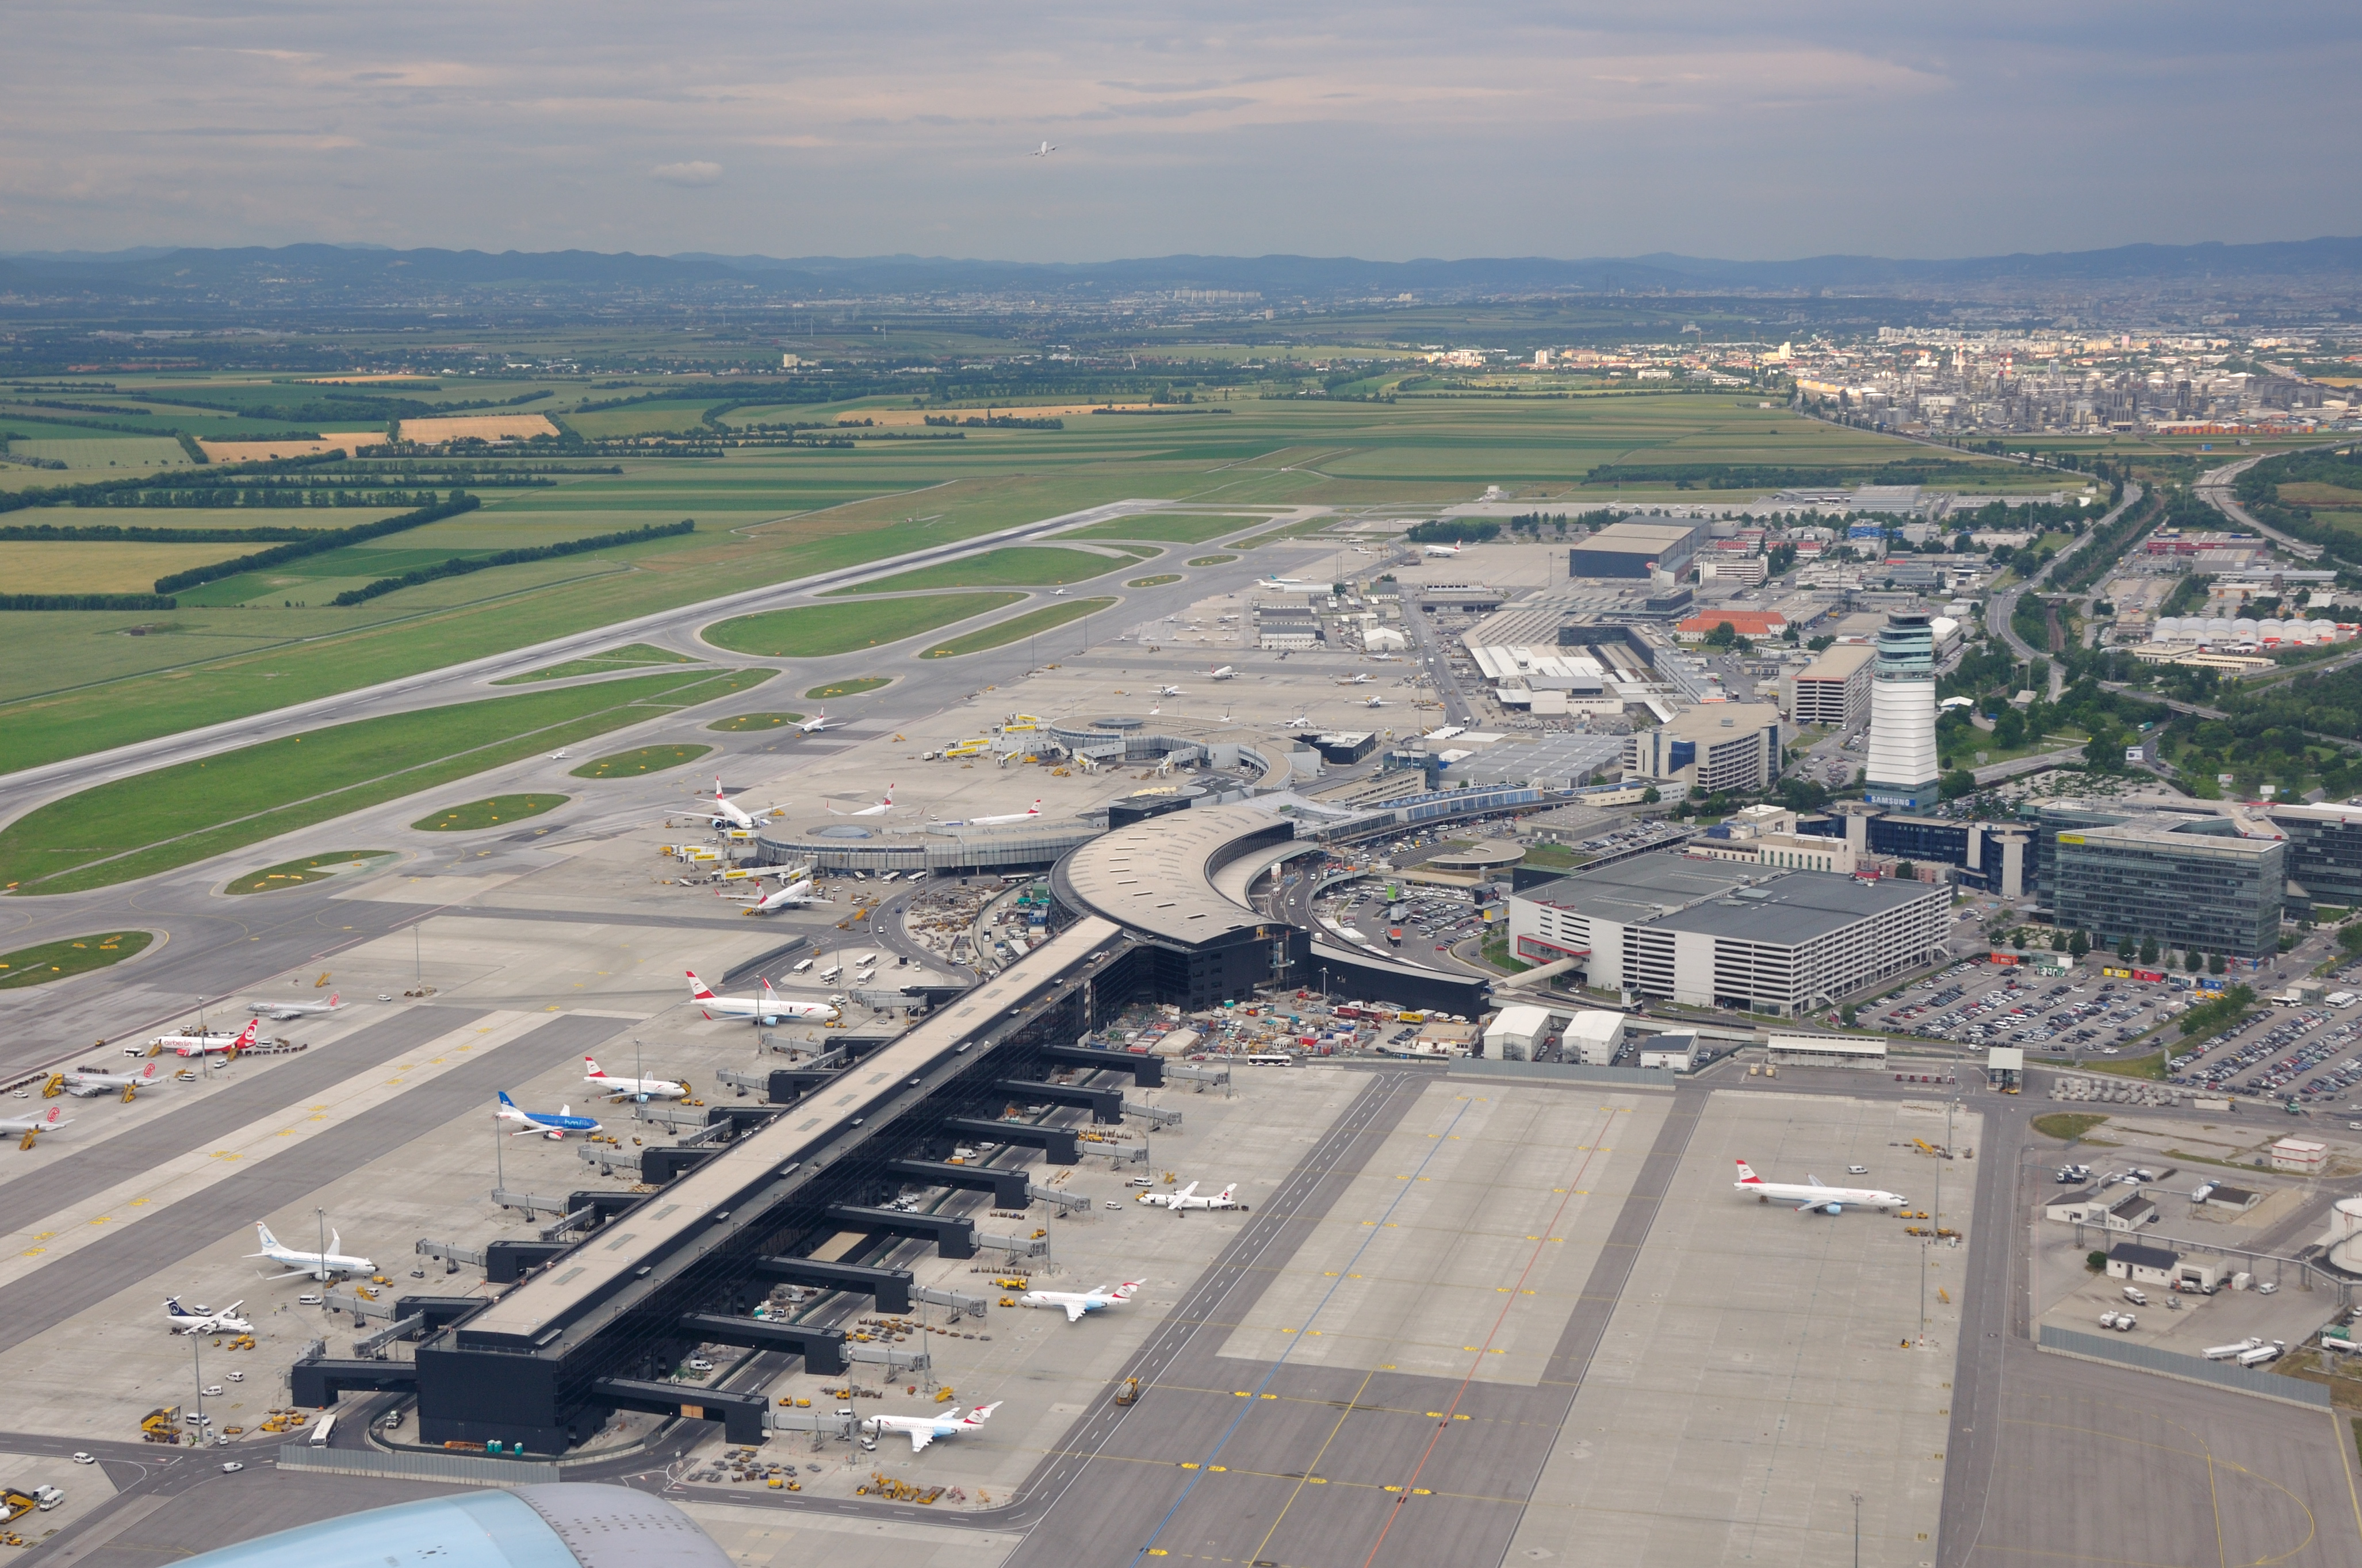
\includegraphics[width=0.7\textwidth]{airport_vienna.jpg}
\footnotesize{Source: Wikipedia}
\end{center}
\end{figure}

\subsubsection*{By Train}
Vienna has good train connections to several European cities and train is the fastest and most convenient
means of transportation between big cities in the region. All trains arrive and depart at the main train
station (Wien Hauptbahnhof).
\begin{description}
\item[\color{kdedarker} Bratislava] -- from Bratislava Hlavná Stanica, hourly, 1~hour, 10 \euro{}
\item[\color{kdedarker} Budapest] -- from Budapest-Keleti, every other hour, 2.75~hours, 19 \euro{}
\item[\color{kdedarker} Prague] -- from Prague Main Station, every other hour, 4~hours, 19 \euro{}
\item[\color{kdedarker} Brno] -- from Brno Main Station, every other hour, 1.5~hours, 9 \euro{}
\end{description}

\subsubsection*{By Bus}
Long-distance bus lines to Vienna are operated by the following companies: Flixbus, Eurolines, StudentAgency (from/to Czech Republic),
Orangeways (from/to Hungary), Polskibus (from/to Poland). If booked in advance, these can offer a cheap alternative to trains or flights.

\subsubsection*{By Car}
Vienna is well-connected to other cities by highways. You can get easily to neighboring countries by car.
Travel time examples:

\begin{description}
\item[\color{kdedarker} Berlin] -- 640 km, 6.75 hours
\item[\color{kdedarker} Budapest] -- 243 km, 2.5 hours
\item[\color{kdedarker} Bratislava] -- 80 km, 1 hour
\item[\color{kdedarker} Prague] -- 300 km, 3.5 hours
\item[\color{kdedarker} Brno] -- 134 km, 1.75 hours
\item[\color{kdedarker} Ljubljana] -- 384 km, 3.75 hours
\item[\color{kdedarker} Zagreb] -- 373 km, 4 hours
\end{description}

Parking near the venue and in most inner districts is not free and only possible for short term. We recommend to park either at your accomodation or in a Park \& Ride garage (Cost: 17 \euro{} for one week).

\subsubsection*{How to get around}
Viennas big public transport system consists of 5 subway lines, tramways, busses and a suburban rail network. The following public transport is reachable in a maximum of 10 minutes walking distance: 
\begin{itemize}
	\item 2 subway stations, Karlsplatz (subway U1, U2, U4) and Taubstummengasse (subway U1) 
	\item Trams \#{1}, \#{2}, \#{62}, \#{71} and D
	\item Bus 59A
\end{itemize}

\vspace{10pt}
Ticket prices (valid for the whole city): 
\begin{itemize}
	\item Single ride: 2,20 \euro{}
	\item 24 hours: 7,60 \euro{}
	\item 48 hours: 13,30 \euro{}
	\item 8 days (do not have to be consecutive): 38,40 \euro{}
	\item Week ticket (Monday till Monday): 16,20 \euro{}
\end{itemize}

\cleardoublepage

\section*{SWAG}
\addcontentsline{toc}{section}{SWAG}
TODO:
We have promotional goods done quite often and have quality and reliable suppliers for swag. Pricing
examples:

\begin{itemize}
\item A~t-shirt with a big logo/picture -- CZK\,87 (\euro{3.55}) if we order 300 t-shirts.
\item Buttons with a logo -- the normal price is CZK\,750 (\euro{30.61}) for 100 pins. If we order for example 
1,000 pins the total price will be CZK\,7,500 (\euro{306}, we may be eligible for a quantity
discount).
\item Stickers -- CZK\,49 (\euro{2}) for an A4 sheet of quality stickers.
\end{itemize}

\cleardoublepage

\section*{The Venue}
\addcontentsline{toc}{section}{The Venue}
The proposed Venue would be the Technical University of Vienna (TU Wien). TU Wien consists of over 10 indivdual buildings, with most of them clustered in the area around Karlsplatz. Out of those buildings, two would fit for Akademy. They are in 5 minutes walking distance, so having the conference days at one and the BoFs at the other would be an option. The location has good public transport connection (see section ''How To Get Around'').\\
Fachschaft Informatik would reserve the necessary rooms, so there would be no reservation fee for them.

\subsection*{Neues EI}
\addcontentsline{toc}{subsection}{Neues EI}

Neues EI (''new electrical-engineering institute'') is a recently renovated building located 10 minutes walking from the subway station Karlsplatz and 5 minutes walking from the subway station Taubstummengasse. Apart from four big lecture rooms on the ground floor, there is a big aula in the building and two areas with computers, that could be used as hacking areas. For the conference it would be the preferred location due to the simple building layout and easy to find rooms. Also it is more representative than Freihaus.

\vspace{10pt}

\begin{wrapfigure}{r}{0.5\textwidth}
\vspace{-22pt}
\begin{center}
\includegraphics[width=0.5\textwidth]{neues_ei_tuwien.jpg}
\footnotesize{Neues EI (Source: TU Wien)}
\end{center}
\vspace{-16pt}
\end{wrapfigure}

Conference \& General Assembly rooms:
\begin{description}
\item[\color{kdedarker} EI7] -- 434 seats, one of the biggest \& most representative lecture rooms at TU Wien.
\item[\color{kdedarker} EI8] -- 139 seats, a lecture room located next to EI7.
\item[\color{kdedarker} EI9] -- 181 seats, a lecture room located around the corner of EI7.
\item[\color{kdedarker} EI10]-- 375 seats, a lecutre room located next to EI9.
\end{description}

\vspace{10pt}
\begin{center}
	\includegraphics[width=0.5\textwidth]{EI7_tuwien.jpg}
	\footnotesize{EI7 (Source: TU Wien)}
\end{center}
\vspace{10pt}

For the BoFs, the following rooms could be used:\\
\begin{itemize}
	\item The 4 lecture rooms from above
	\item An additional lecutre room in the 3rd floor
	\item Up to 8 seminar rooms on the 2nd to 4th floor
\end{itemize}

Due to the scattered seminar rooms, the other location would be a better fit for the BoFs.

\subsubsection*{Equipment}
\addcontentsline{toc}{subsubsection}{Equipment}
All lecture \& seminar rooms are equipped with:
\begin{itemize}
	\item a projector,
	\item a cable to connect a laptop to the projector,
	\item audio (hands-free microphones),
	\item video and audio recording,
	\item wifi connection (encrypted, guest accounts would need to be organized)
\end{itemize}

The entire building is covered by a wireless network.

\newpage

\subsection*{Freihaus}
\addcontentsline{toc}{subsection}{Freihaus}
TODO: everything except equipment\\
NOTES: BoF rooms: FH2, 3, 4, Fachgruppenraum Physik, ZID Räume

There faculty has three big lecture rooms:
\begin{description}
\item[\color{kdedarker} D1] -- 248 seats
\item[\color{kdedarker} D2] -- 122 seats
\item[\color{kdedarker} D3] -- 179 seats
\end{description}

There are also many smaller lecture rooms and class rooms that could be used for BoF sessions.

\subsubsection*{Equipment}
\addcontentsline{toc}{subsubsection}{Equipment}
All lecture \& seminar rooms are equipped with:
\begin{itemize}
\item a projector,
\item a cable to connect a laptop to the projector,
\item audio (hands-free microphones),
\item video and audio recording,
\item wifi connection (encrypted, guest accounts would need to be organized)
\end{itemize}

The entire building is covered by a wireless network.

\begin{figure}[ht]
\centering
% \subfloat{\includegraphics[width=0.49\textwidth]{fimu1.jpg}}\hfill
% \subfloat{\includegraphics[width=0.49\textwidth]{fimu2.jpg}}
\end{figure}



\subsection*{Catering}
\addcontentsline{toc}{subsection}{Catering}
TODO:
There is no cafeteria in the building, but there are several restaurants around the faculty:

\begin{description}
\item[\color{kdedarker} Al Capone] -- italian restaurant, offers several vegatarian meals -- \sloppy \mbox{\url{www.pizzaalcapone.cz}}
\item[\color{kdedarker} Magistr] -- a microbrewery with restarurant -- \url{www.pivovarmagistr.cz}
\item[\color{kdedarker} AURA restaurant] -- restaurant, cafe, bar -- \url{www.campea.cz}
\item[\color{kdedarker} Catering On Site] -- basic catering (mineral water, hot
beverages, snacks) could be provided on site, so that attendants can get refreshment
between talks
\end{description}


\newpage

\section*{Social Events}
\addcontentsline{toc}{section}{Social Events}
TODO: 

\begin{wrapfigure}{r}{0.3\textwidth}
\vspace{-22pt}
\begin{center}
% \includegraphics[width=0.3\textwidth]{fleda.jpg}
\footnotesize{Source: Michal Sänger - BY-CN-SA}
\vspace{-20pt}
\end{center}
\end{wrapfigure}

Brno offers good venues to organize conference parties. Some of them are
really close to the proposed conference venue. Here are some we propose
because we've already organized social events there and have good
experience with them:

\begin{description}
\item[\color{kdedarker} Fléda] -- a large venue for concerts and other events which is located
30 minutes walk from the conference venue. It has capacity up to 800 people.
The rent for one night is CZK\,31,700 (\euro{1,230}) and can provide discount
on catering. Fléda website: \url{http://www.fleda.cz}
\item[\color{kdedarker} Semilasso] -- venue for concerts and other events which is
just a few hundred meters from the conference venue. The main hall
has capacity 700 people, the garden 300 people. The rent for one night
is CZK\,35,000 (\euro{1,355}). The club is also suitable for concerts,
both outside and inside. The club's website:
\url{http://www.semilasso.cz/}
\item[\color{kdedarker} Brewery Brno] -- a large restaurant located on the premises of
Brno's brewery. The capacity of the main hall is at least 300 people.
It has a dance floor and a DJ can be arranged. A~rent for one night is
CZK\,90,000 (\euro{3,673}). The rent is free if you order catering. The
restaurant's website:
\url{http://www.pivovarskabrno.cz/}
\end{description}

\cleardoublepage

\section*{Accomodation}
\addcontentsline{toc}{section}{Accomodation}
TODO:
We'd like to provide several price levels of accommodation to suit to all conference attendants:

\subsection*{Low Cost}
\addcontentsline{toc}{subsection}{Low Cost}
\begin{itemize}
\item \emph{Student Dormitories} of the Mendel University in Brno -- 
are the cheapest accommodation option. They can provide a
large number of rooms. The current price is CZK\,600 (\euro{23.3}) for a
double-bed room and CZK\,400 (\euro{15.5}) for single-bed room. Breakfast is additional
CZK\,110 (\euro{4.3}). The dormitories have facilities
such as a student cafeteria, pizzeria, sport facilities, and even a
cinema. The campus is just 3~bus stops away from the venue and the bus
53 takes you almost from door to door. If you feel like stretching your
legs a bit the pleasent walk will take you about 15 -- 20 minutes. A~tram
takes you to the old town in about 20 minutes.
\end{itemize}

\begin{figure}[ht]
\begin{center}
% \includegraphics[width=0.6\textwidth]{tauferky.jpg}
\end{center}
\end{figure}

\subsection*{Mid-Range}
\addcontentsline{toc}{subsection}{Mid-Range}
\begin{itemize}
\item \emph{Hotel Avanti} $\star\star\star\star{}$ -- is another mid-range option we recommend. One
double bed room is CZK\,1,690 (\euro{69}) for one person and CZK\,1,840
(\euro{75} for two persons). The hotel also offers more expensive
options up to a President suite for CZK\,4,890 (\euro{200}). It might be possible
to arrange a discount for Akademy attendees. The hotel is 15
minutes (tram), 25 minutes (walking) from the conference venue. And it's
just 12 minutes by tram to get to the city center. The hotel's website:
\url{http://www.brno-hotel-avanti.eu/}
\end{itemize}


\begin{figure}[ht]
\begin{center}
% \includegraphics[width=0.7\textwidth]{avanti.jpg}
\end{center}
\end{figure}

\subsection*{High-end}
\addcontentsline{toc}{subsection}{High-end}
\begin{itemize}
\item \emph{Barceló Brno Palace} $\star\star\star\star{}$+ -- the newest and one of the most luxurious hotels in Brno
has airy interior with Spanish-style design and a very good restaurant. It satisfies the highest
standards. Rooms start at \euro{137}. It takes 10 minutes by car (20 minutes by tram) to get from
the hotel to the venue, the city center is just a few minutes of walking away. The hotel's web-
site: \sloppy \url{http://www.barcelobrnopalace.com/BarceloHotels/en\_GB/hotels/Czech-Republic/Brno/
hotel-barcelo-brno-palace/general-description.aspx}
\end{itemize}

\begin{figure}[ht]
\begin{center}
% \includegraphics[width=0.7\textwidth]{barcelo.jpg}
\end{center}
\end{figure}

\section*{Acknowledgements}
\addcontentsline{toc}{section}{Acknowledgements}

\begin{description}
	\item[\color{kdedarker} Daniel Vrátil] -- for providing us with the LaTeX source of the Akademy 2014 proposal
	\item[\color{kdedarker} Albert Astals Cid \& Aleix Pol] -- for answering quite a few questions about the proposal
\end{description}

\cleardoublepage

\section*{Contact}
\addcontentsline{toc}{section}{Contact}
\Author

\end{document}
